% Graphic for TeX using PGF
% Title: /home/tobias/Documents/HSLU/NS/I_BA_NS1701/Termpaper/Klassendiagramm.dia
% Creator: Dia v0.97.3
% CreationDate: Thu May  4 09:03:17 2017
% For: tobias
% \usepackage{tikz}
% The following commands are not supported in PSTricks at present
% We define them conditionally, so when they are implemented,
% this pgf file will use them.
\ifx\du\undefined
  \newlength{\du}
\fi
\setlength{\du}{15\unitlength}
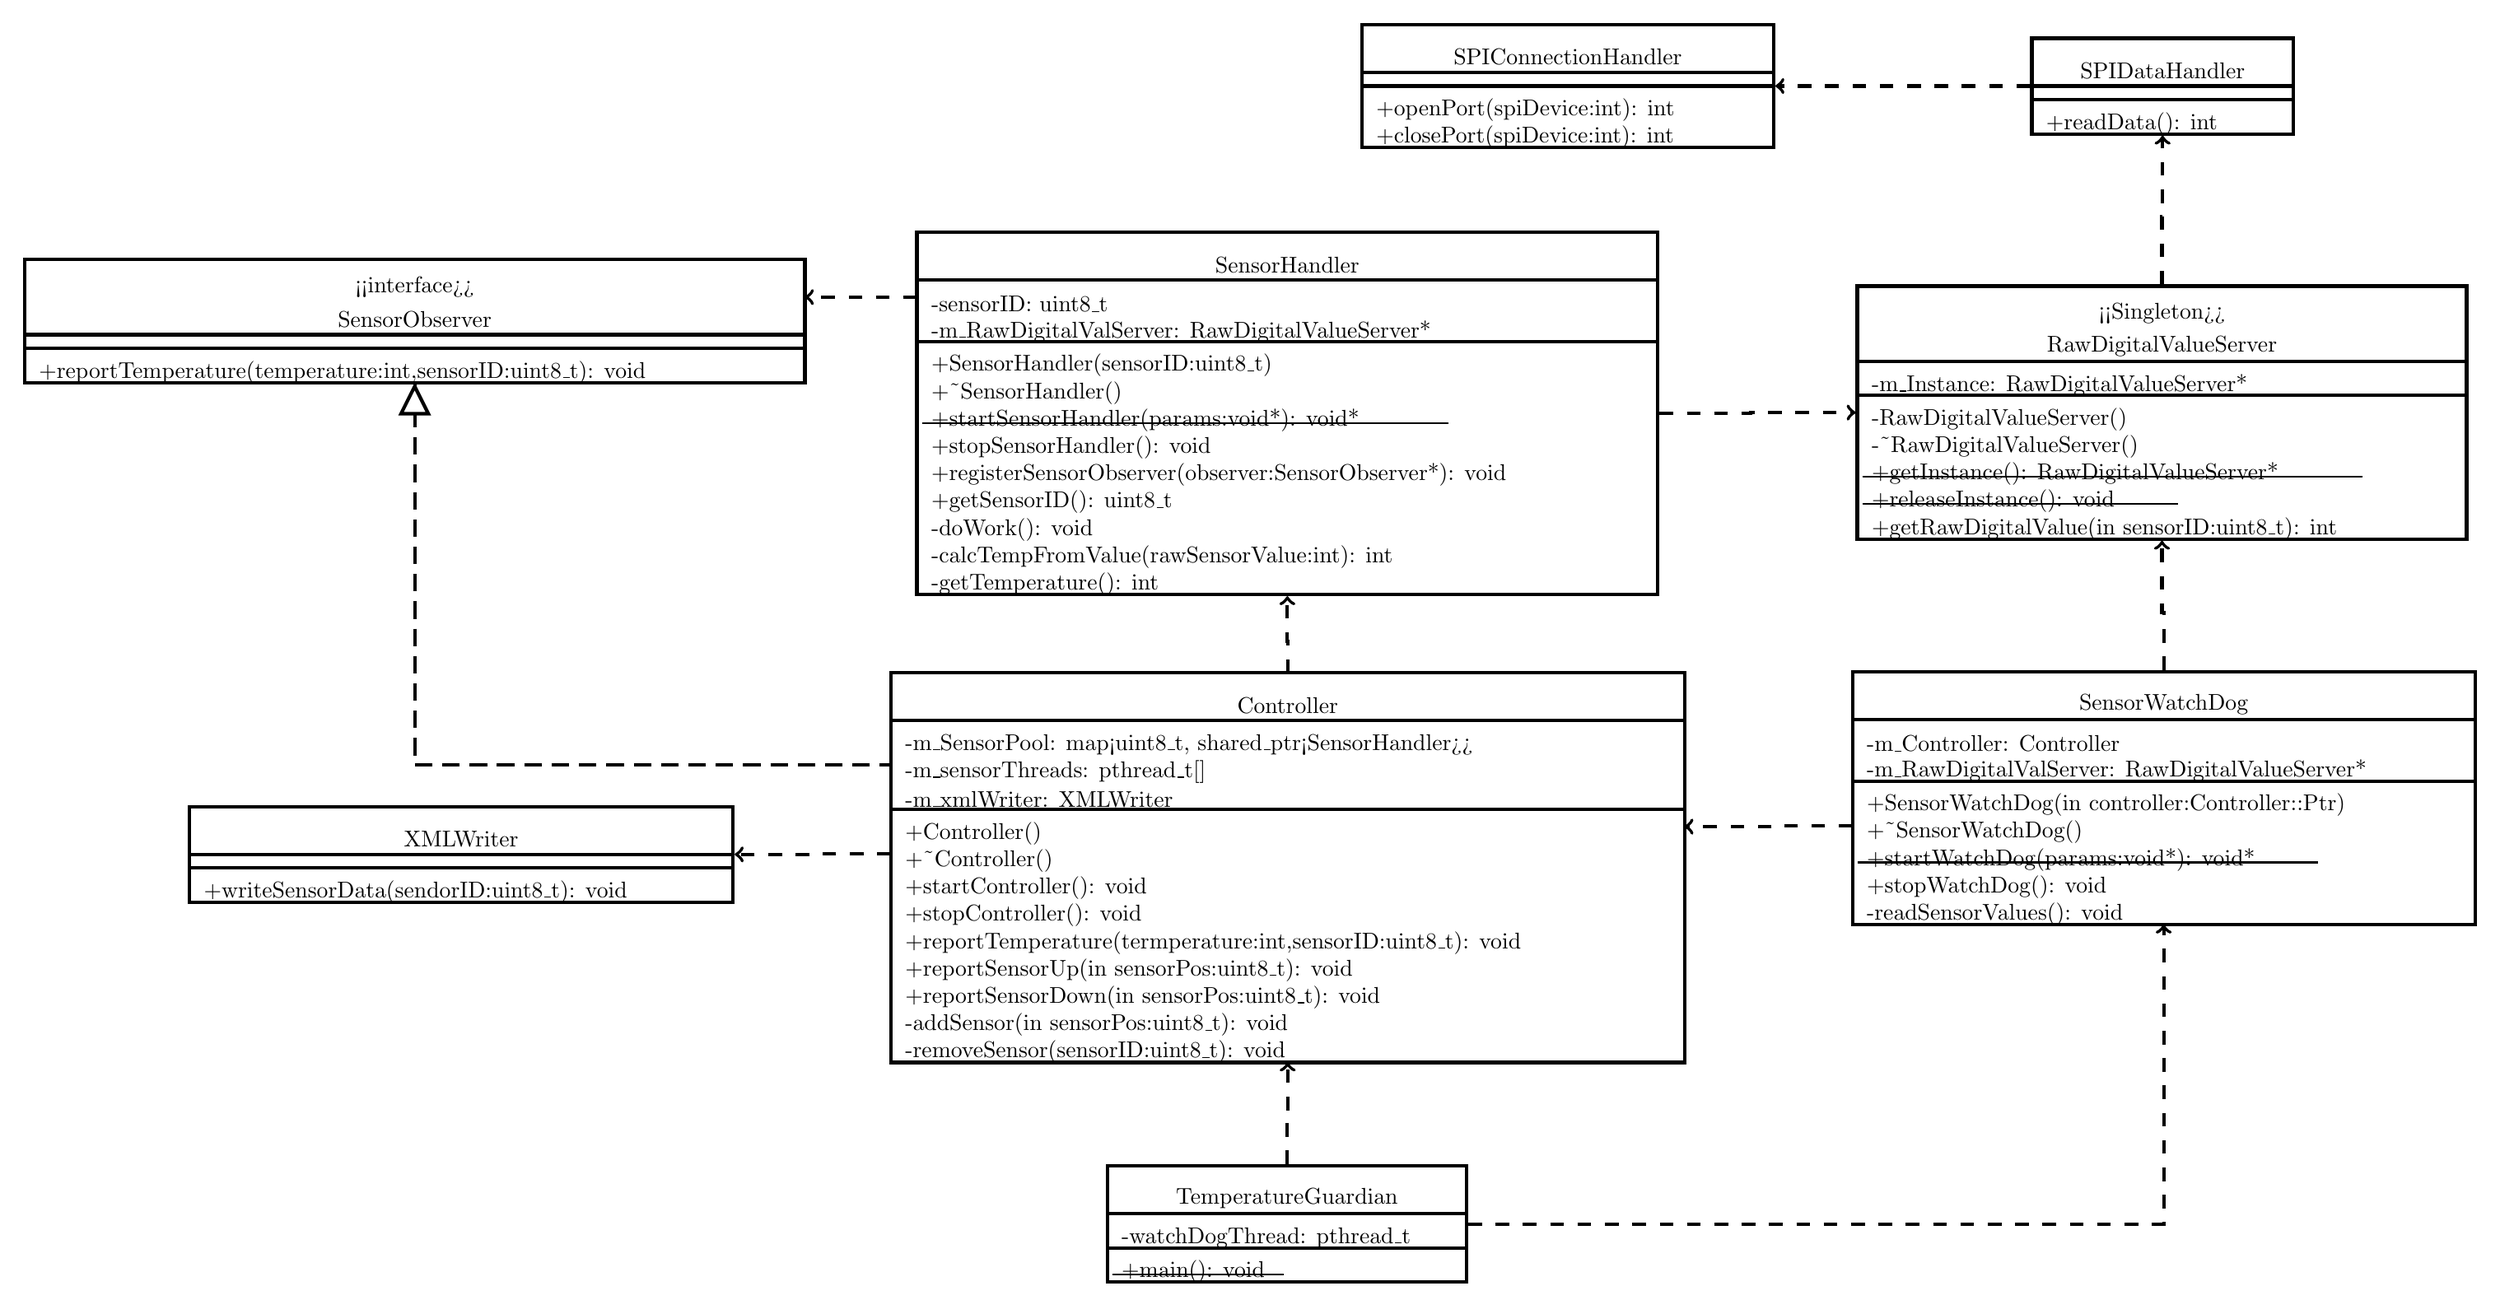
\begin{tikzpicture}
\pgftransformxscale{1.000000}
\pgftransformyscale{-1.000000}
\definecolor{dialinecolor}{rgb}{0.000000, 0.000000, 0.000000}
\pgfsetstrokecolor{dialinecolor}
\definecolor{dialinecolor}{rgb}{1.000000, 1.000000, 1.000000}
\pgfsetfillcolor{dialinecolor}
\pgfsetlinewidth{0.100000\du}
\pgfsetdash{}{0pt}
\definecolor{dialinecolor}{rgb}{1.000000, 1.000000, 1.000000}
\pgfsetfillcolor{dialinecolor}
\fill (11.811300\du,38.069200\du)--(11.811300\du,39.469200\du)--(22.321300\du,39.469200\du)--(22.321300\du,38.069200\du)--cycle;
\definecolor{dialinecolor}{rgb}{0.000000, 0.000000, 0.000000}
\pgfsetstrokecolor{dialinecolor}
\draw (11.811300\du,38.069200\du)--(11.811300\du,39.469200\du)--(22.321300\du,39.469200\du)--(22.321300\du,38.069200\du)--cycle;
% setfont left to latex
\definecolor{dialinecolor}{rgb}{0.000000, 0.000000, 0.000000}
\pgfsetstrokecolor{dialinecolor}
\node at (17.066300\du,39.019200\du){TemperatureGuardian};
\definecolor{dialinecolor}{rgb}{1.000000, 1.000000, 1.000000}
\pgfsetfillcolor{dialinecolor}
\fill (11.811300\du,39.469200\du)--(11.811300\du,40.469200\du)--(22.321300\du,40.469200\du)--(22.321300\du,39.469200\du)--cycle;
\definecolor{dialinecolor}{rgb}{0.000000, 0.000000, 0.000000}
\pgfsetstrokecolor{dialinecolor}
\draw (11.811300\du,39.469200\du)--(11.811300\du,40.469200\du)--(22.321300\du,40.469200\du)--(22.321300\du,39.469200\du)--cycle;
% setfont left to latex
\definecolor{dialinecolor}{rgb}{0.000000, 0.000000, 0.000000}
\pgfsetstrokecolor{dialinecolor}
\node[anchor=west] at (11.961300\du,40.169200\du){-watchDogThread: pthread\_t};
\definecolor{dialinecolor}{rgb}{1.000000, 1.000000, 1.000000}
\pgfsetfillcolor{dialinecolor}
\fill (11.811300\du,40.469200\du)--(11.811300\du,41.469200\du)--(22.321300\du,41.469200\du)--(22.321300\du,40.469200\du)--cycle;
\definecolor{dialinecolor}{rgb}{0.000000, 0.000000, 0.000000}
\pgfsetstrokecolor{dialinecolor}
\draw (11.811300\du,40.469200\du)--(11.811300\du,41.469200\du)--(22.321300\du,41.469200\du)--(22.321300\du,40.469200\du)--cycle;
% setfont left to latex
\definecolor{dialinecolor}{rgb}{0.000000, 0.000000, 0.000000}
\pgfsetstrokecolor{dialinecolor}
\node[anchor=west] at (11.961300\du,41.169200\du){+main(): void};
\pgfsetlinewidth{0.050000\du}
\definecolor{dialinecolor}{rgb}{0.000000, 0.000000, 0.000000}
\pgfsetstrokecolor{dialinecolor}
\draw (11.961300\du,41.249200\du)--(16.966300\du,41.249200\du);
\pgfsetlinewidth{0.100000\du}
\pgfsetlinewidth{0.100000\du}
\pgfsetdash{}{0pt}
\definecolor{dialinecolor}{rgb}{1.000000, 1.000000, 1.000000}
\pgfsetfillcolor{dialinecolor}
\fill (5.480760\du,23.642600\du)--(5.480760\du,25.042600\du)--(28.695760\du,25.042600\du)--(28.695760\du,23.642600\du)--cycle;
\definecolor{dialinecolor}{rgb}{0.000000, 0.000000, 0.000000}
\pgfsetstrokecolor{dialinecolor}
\draw (5.480760\du,23.642600\du)--(5.480760\du,25.042600\du)--(28.695760\du,25.042600\du)--(28.695760\du,23.642600\du)--cycle;
% setfont left to latex
\definecolor{dialinecolor}{rgb}{0.000000, 0.000000, 0.000000}
\pgfsetstrokecolor{dialinecolor}
\node at (17.088260\du,24.592600\du){Controller};
\definecolor{dialinecolor}{rgb}{1.000000, 1.000000, 1.000000}
\pgfsetfillcolor{dialinecolor}
\fill (5.480760\du,25.042600\du)--(5.480760\du,27.642600\du)--(28.695760\du,27.642600\du)--(28.695760\du,25.042600\du)--cycle;
\definecolor{dialinecolor}{rgb}{0.000000, 0.000000, 0.000000}
\pgfsetstrokecolor{dialinecolor}
\draw (5.480760\du,25.042600\du)--(5.480760\du,27.642600\du)--(28.695760\du,27.642600\du)--(28.695760\du,25.042600\du)--cycle;
% setfont left to latex
\definecolor{dialinecolor}{rgb}{0.000000, 0.000000, 0.000000}
\pgfsetstrokecolor{dialinecolor}
\node[anchor=west] at (5.630760\du,25.742600\du){-m\_SensorPool: map<uint8\_t, shared\_ptr<SensorHandler>>};
% setfont left to latex
\definecolor{dialinecolor}{rgb}{0.000000, 0.000000, 0.000000}
\pgfsetstrokecolor{dialinecolor}
\node[anchor=west] at (5.630760\du,26.542600\du){-m\_sensorThreads: pthread\_t\ensuremath{[}\ensuremath{]}};
% setfont left to latex
\definecolor{dialinecolor}{rgb}{0.000000, 0.000000, 0.000000}
\pgfsetstrokecolor{dialinecolor}
\node[anchor=west] at (5.630760\du,27.342600\du){-m\_xmlWriter: XMLWriter};
\definecolor{dialinecolor}{rgb}{1.000000, 1.000000, 1.000000}
\pgfsetfillcolor{dialinecolor}
\fill (5.480760\du,27.642600\du)--(5.480760\du,35.042600\du)--(28.695760\du,35.042600\du)--(28.695760\du,27.642600\du)--cycle;
\definecolor{dialinecolor}{rgb}{0.000000, 0.000000, 0.000000}
\pgfsetstrokecolor{dialinecolor}
\draw (5.480760\du,27.642600\du)--(5.480760\du,35.042600\du)--(28.695760\du,35.042600\du)--(28.695760\du,27.642600\du)--cycle;
% setfont left to latex
\definecolor{dialinecolor}{rgb}{0.000000, 0.000000, 0.000000}
\pgfsetstrokecolor{dialinecolor}
\node[anchor=west] at (5.630760\du,28.342600\du){+Controller()};
% setfont left to latex
\definecolor{dialinecolor}{rgb}{0.000000, 0.000000, 0.000000}
\pgfsetstrokecolor{dialinecolor}
\node[anchor=west] at (5.630760\du,29.142600\du){+\~{}Controller()};
% setfont left to latex
\definecolor{dialinecolor}{rgb}{0.000000, 0.000000, 0.000000}
\pgfsetstrokecolor{dialinecolor}
\node[anchor=west] at (5.630760\du,29.942600\du){+startController(): void};
% setfont left to latex
\definecolor{dialinecolor}{rgb}{0.000000, 0.000000, 0.000000}
\pgfsetstrokecolor{dialinecolor}
\node[anchor=west] at (5.630760\du,30.742600\du){+stopController(): void};
% setfont left to latex
\definecolor{dialinecolor}{rgb}{0.000000, 0.000000, 0.000000}
\pgfsetstrokecolor{dialinecolor}
\node[anchor=west] at (5.630760\du,31.542600\du){+reportTemperature(termperature:int,sensorID:uint8\_t): void};
% setfont left to latex
\definecolor{dialinecolor}{rgb}{0.000000, 0.000000, 0.000000}
\pgfsetstrokecolor{dialinecolor}
\node[anchor=west] at (5.630760\du,32.342600\du){+reportSensorUp(in sensorPos:uint8\_t): void};
% setfont left to latex
\definecolor{dialinecolor}{rgb}{0.000000, 0.000000, 0.000000}
\pgfsetstrokecolor{dialinecolor}
\node[anchor=west] at (5.630760\du,33.142600\du){+reportSensorDown(in sensorPos:uint8\_t): void};
% setfont left to latex
\definecolor{dialinecolor}{rgb}{0.000000, 0.000000, 0.000000}
\pgfsetstrokecolor{dialinecolor}
\node[anchor=west] at (5.630760\du,33.942600\du){-addSensor(in sensorPos:uint8\_t): void};
% setfont left to latex
\definecolor{dialinecolor}{rgb}{0.000000, 0.000000, 0.000000}
\pgfsetstrokecolor{dialinecolor}
\node[anchor=west] at (5.630760\du,34.742600\du){-removeSensor(sensorID:uint8\_t): void};
\pgfsetlinewidth{0.100000\du}
\pgfsetdash{{1.000000\du}{1.000000\du}}{0\du}
\pgfsetdash{{0.400000\du}{0.400000\du}}{0\du}
\pgfsetmiterjoin
\pgfsetbuttcap
{
\definecolor{dialinecolor}{rgb}{0.000000, 0.000000, 0.000000}
\pgfsetfillcolor{dialinecolor}
% was here!!!
\pgfsetarrowsend{to}
\definecolor{dialinecolor}{rgb}{0.000000, 0.000000, 0.000000}
\pgfsetstrokecolor{dialinecolor}
\draw (17.066300\du,38.018773\du)--(17.066300\du,36.730686\du)--(17.088260\du,36.730686\du)--(17.088260\du,35.042600\du);
}
% setfont left to latex
\pgfsetlinewidth{0.100000\du}
\pgfsetdash{}{0pt}
\definecolor{dialinecolor}{rgb}{1.000000, 1.000000, 1.000000}
\pgfsetfillcolor{dialinecolor}
\fill (6.242280\du,10.750000\du)--(6.242280\du,12.150000\du)--(27.917280\du,12.150000\du)--(27.917280\du,10.750000\du)--cycle;
\definecolor{dialinecolor}{rgb}{0.000000, 0.000000, 0.000000}
\pgfsetstrokecolor{dialinecolor}
\draw (6.242280\du,10.750000\du)--(6.242280\du,12.150000\du)--(27.917280\du,12.150000\du)--(27.917280\du,10.750000\du)--cycle;
% setfont left to latex
\definecolor{dialinecolor}{rgb}{0.000000, 0.000000, 0.000000}
\pgfsetstrokecolor{dialinecolor}
\node at (17.079780\du,11.700000\du){SensorHandler};
\definecolor{dialinecolor}{rgb}{1.000000, 1.000000, 1.000000}
\pgfsetfillcolor{dialinecolor}
\fill (6.242280\du,12.150000\du)--(6.242280\du,13.950000\du)--(27.917280\du,13.950000\du)--(27.917280\du,12.150000\du)--cycle;
\definecolor{dialinecolor}{rgb}{0.000000, 0.000000, 0.000000}
\pgfsetstrokecolor{dialinecolor}
\draw (6.242280\du,12.150000\du)--(6.242280\du,13.950000\du)--(27.917280\du,13.950000\du)--(27.917280\du,12.150000\du)--cycle;
% setfont left to latex
\definecolor{dialinecolor}{rgb}{0.000000, 0.000000, 0.000000}
\pgfsetstrokecolor{dialinecolor}
\node[anchor=west] at (6.392280\du,12.850000\du){-sensorID: uint8\_t};
% setfont left to latex
\definecolor{dialinecolor}{rgb}{0.000000, 0.000000, 0.000000}
\pgfsetstrokecolor{dialinecolor}
\node[anchor=west] at (6.392280\du,13.650000\du){-m\_RawDigitalValServer: RawDigitalValueServer*};
\definecolor{dialinecolor}{rgb}{1.000000, 1.000000, 1.000000}
\pgfsetfillcolor{dialinecolor}
\fill (6.242280\du,13.950000\du)--(6.242280\du,21.350000\du)--(27.917280\du,21.350000\du)--(27.917280\du,13.950000\du)--cycle;
\definecolor{dialinecolor}{rgb}{0.000000, 0.000000, 0.000000}
\pgfsetstrokecolor{dialinecolor}
\draw (6.242280\du,13.950000\du)--(6.242280\du,21.350000\du)--(27.917280\du,21.350000\du)--(27.917280\du,13.950000\du)--cycle;
% setfont left to latex
\definecolor{dialinecolor}{rgb}{0.000000, 0.000000, 0.000000}
\pgfsetstrokecolor{dialinecolor}
\node[anchor=west] at (6.392280\du,14.650000\du){+SensorHandler(sensorID:uint8\_t)};
% setfont left to latex
\definecolor{dialinecolor}{rgb}{0.000000, 0.000000, 0.000000}
\pgfsetstrokecolor{dialinecolor}
\node[anchor=west] at (6.392280\du,15.450000\du){+\~{}SensorHandler()};
% setfont left to latex
\definecolor{dialinecolor}{rgb}{0.000000, 0.000000, 0.000000}
\pgfsetstrokecolor{dialinecolor}
\node[anchor=west] at (6.392280\du,16.250000\du){+startSensorHandler(params:void*): void*};
\pgfsetlinewidth{0.050000\du}
\definecolor{dialinecolor}{rgb}{0.000000, 0.000000, 0.000000}
\pgfsetstrokecolor{dialinecolor}
\draw (6.392280\du,16.330000\du)--(21.792280\du,16.330000\du);
\pgfsetlinewidth{0.100000\du}
% setfont left to latex
\definecolor{dialinecolor}{rgb}{0.000000, 0.000000, 0.000000}
\pgfsetstrokecolor{dialinecolor}
\node[anchor=west] at (6.392280\du,17.050000\du){+stopSensorHandler(): void};
% setfont left to latex
\definecolor{dialinecolor}{rgb}{0.000000, 0.000000, 0.000000}
\pgfsetstrokecolor{dialinecolor}
\node[anchor=west] at (6.392280\du,17.850000\du){+registerSensorObserver(observer:SensorObserver*): void};
% setfont left to latex
\definecolor{dialinecolor}{rgb}{0.000000, 0.000000, 0.000000}
\pgfsetstrokecolor{dialinecolor}
\node[anchor=west] at (6.392280\du,18.650000\du){+getSensorID(): uint8\_t};
% setfont left to latex
\definecolor{dialinecolor}{rgb}{0.000000, 0.000000, 0.000000}
\pgfsetstrokecolor{dialinecolor}
\node[anchor=west] at (6.392280\du,19.450000\du){-doWork(): void};
% setfont left to latex
\definecolor{dialinecolor}{rgb}{0.000000, 0.000000, 0.000000}
\pgfsetstrokecolor{dialinecolor}
\node[anchor=west] at (6.392280\du,20.250000\du){-calcTempFromValue(rawSensorValue:int): int};
% setfont left to latex
\definecolor{dialinecolor}{rgb}{0.000000, 0.000000, 0.000000}
\pgfsetstrokecolor{dialinecolor}
\node[anchor=west] at (6.392280\du,21.050000\du){-getTemperature(): int};
\pgfsetlinewidth{0.100000\du}
\pgfsetdash{}{0pt}
\definecolor{dialinecolor}{rgb}{1.000000, 1.000000, 1.000000}
\pgfsetfillcolor{dialinecolor}
\fill (33.753800\du,12.326900\du)--(33.753800\du,14.526900\du)--(51.578800\du,14.526900\du)--(51.578800\du,12.326900\du)--cycle;
\definecolor{dialinecolor}{rgb}{0.000000, 0.000000, 0.000000}
\pgfsetstrokecolor{dialinecolor}
\draw (33.753800\du,12.326900\du)--(33.753800\du,14.526900\du)--(51.578800\du,14.526900\du)--(51.578800\du,12.326900\du)--cycle;
% setfont left to latex
\definecolor{dialinecolor}{rgb}{0.000000, 0.000000, 0.000000}
\pgfsetstrokecolor{dialinecolor}
\node at (42.666300\du,13.126900\du){<<Singleton>>};
% setfont left to latex
\definecolor{dialinecolor}{rgb}{0.000000, 0.000000, 0.000000}
\pgfsetstrokecolor{dialinecolor}
\node at (42.666300\du,14.076900\du){RawDigitalValueServer};
\definecolor{dialinecolor}{rgb}{1.000000, 1.000000, 1.000000}
\pgfsetfillcolor{dialinecolor}
\fill (33.753800\du,14.526900\du)--(33.753800\du,15.526900\du)--(51.578800\du,15.526900\du)--(51.578800\du,14.526900\du)--cycle;
\definecolor{dialinecolor}{rgb}{0.000000, 0.000000, 0.000000}
\pgfsetstrokecolor{dialinecolor}
\draw (33.753800\du,14.526900\du)--(33.753800\du,15.526900\du)--(51.578800\du,15.526900\du)--(51.578800\du,14.526900\du)--cycle;
% setfont left to latex
\definecolor{dialinecolor}{rgb}{0.000000, 0.000000, 0.000000}
\pgfsetstrokecolor{dialinecolor}
\node[anchor=west] at (33.903800\du,15.226900\du){-m\_Instance: RawDigitalValueServer*};
\pgfsetlinewidth{0.050000\du}
\definecolor{dialinecolor}{rgb}{0.000000, 0.000000, 0.000000}
\pgfsetstrokecolor{dialinecolor}
\draw (33.903800\du,15.506900\du)--(47.378800\du,15.506900\du);
\pgfsetlinewidth{0.100000\du}
\definecolor{dialinecolor}{rgb}{1.000000, 1.000000, 1.000000}
\pgfsetfillcolor{dialinecolor}
\fill (33.753800\du,15.526900\du)--(33.753800\du,19.726900\du)--(51.578800\du,19.726900\du)--(51.578800\du,15.526900\du)--cycle;
\definecolor{dialinecolor}{rgb}{0.000000, 0.000000, 0.000000}
\pgfsetstrokecolor{dialinecolor}
\draw (33.753800\du,15.526900\du)--(33.753800\du,19.726900\du)--(51.578800\du,19.726900\du)--(51.578800\du,15.526900\du)--cycle;
% setfont left to latex
\definecolor{dialinecolor}{rgb}{0.000000, 0.000000, 0.000000}
\pgfsetstrokecolor{dialinecolor}
\node[anchor=west] at (33.903800\du,16.226900\du){-RawDigitalValueServer()};
% setfont left to latex
\definecolor{dialinecolor}{rgb}{0.000000, 0.000000, 0.000000}
\pgfsetstrokecolor{dialinecolor}
\node[anchor=west] at (33.903800\du,17.026900\du){-\~{}RawDigitalValueServer()};
% setfont left to latex
\definecolor{dialinecolor}{rgb}{0.000000, 0.000000, 0.000000}
\pgfsetstrokecolor{dialinecolor}
\node[anchor=west] at (33.903800\du,17.826900\du){+getInstance(): RawDigitalValueServer*};
\pgfsetlinewidth{0.050000\du}
\definecolor{dialinecolor}{rgb}{0.000000, 0.000000, 0.000000}
\pgfsetstrokecolor{dialinecolor}
\draw (33.903800\du,17.906900\du)--(48.533800\du,17.906900\du);
\pgfsetlinewidth{0.100000\du}
% setfont left to latex
\definecolor{dialinecolor}{rgb}{0.000000, 0.000000, 0.000000}
\pgfsetstrokecolor{dialinecolor}
\node[anchor=west] at (33.903800\du,18.626900\du){+releaseInstance(): void};
\pgfsetlinewidth{0.050000\du}
\definecolor{dialinecolor}{rgb}{0.000000, 0.000000, 0.000000}
\pgfsetstrokecolor{dialinecolor}
\draw (33.903800\du,18.706900\du)--(43.143800\du,18.706900\du);
\pgfsetlinewidth{0.100000\du}
% setfont left to latex
\definecolor{dialinecolor}{rgb}{0.000000, 0.000000, 0.000000}
\pgfsetstrokecolor{dialinecolor}
\node[anchor=west] at (33.903800\du,19.426900\du){+getRawDigitalValue(in sensorID:uint8\_t): int};
\pgfsetlinewidth{0.100000\du}
\pgfsetdash{}{0pt}
\definecolor{dialinecolor}{rgb}{1.000000, 1.000000, 1.000000}
\pgfsetfillcolor{dialinecolor}
\fill (33.611500\du,23.609300\du)--(33.611500\du,25.009300\du)--(51.821500\du,25.009300\du)--(51.821500\du,23.609300\du)--cycle;
\definecolor{dialinecolor}{rgb}{0.000000, 0.000000, 0.000000}
\pgfsetstrokecolor{dialinecolor}
\draw (33.611500\du,23.609300\du)--(33.611500\du,25.009300\du)--(51.821500\du,25.009300\du)--(51.821500\du,23.609300\du)--cycle;
% setfont left to latex
\definecolor{dialinecolor}{rgb}{0.000000, 0.000000, 0.000000}
\pgfsetstrokecolor{dialinecolor}
\node at (42.716500\du,24.559300\du){SensorWatchDog};
\definecolor{dialinecolor}{rgb}{1.000000, 1.000000, 1.000000}
\pgfsetfillcolor{dialinecolor}
\fill (33.611500\du,25.009300\du)--(33.611500\du,26.809300\du)--(51.821500\du,26.809300\du)--(51.821500\du,25.009300\du)--cycle;
\definecolor{dialinecolor}{rgb}{0.000000, 0.000000, 0.000000}
\pgfsetstrokecolor{dialinecolor}
\draw (33.611500\du,25.009300\du)--(33.611500\du,26.809300\du)--(51.821500\du,26.809300\du)--(51.821500\du,25.009300\du)--cycle;
% setfont left to latex
\definecolor{dialinecolor}{rgb}{0.000000, 0.000000, 0.000000}
\pgfsetstrokecolor{dialinecolor}
\node[anchor=west] at (33.761500\du,25.709300\du){-m\_Controller: Controller};
% setfont left to latex
\definecolor{dialinecolor}{rgb}{0.000000, 0.000000, 0.000000}
\pgfsetstrokecolor{dialinecolor}
\node[anchor=west] at (33.761500\du,26.509300\du){-m\_RawDigitalValServer: RawDigitalValueServer*};
\definecolor{dialinecolor}{rgb}{1.000000, 1.000000, 1.000000}
\pgfsetfillcolor{dialinecolor}
\fill (33.611500\du,26.809300\du)--(33.611500\du,31.009300\du)--(51.821500\du,31.009300\du)--(51.821500\du,26.809300\du)--cycle;
\definecolor{dialinecolor}{rgb}{0.000000, 0.000000, 0.000000}
\pgfsetstrokecolor{dialinecolor}
\draw (33.611500\du,26.809300\du)--(33.611500\du,31.009300\du)--(51.821500\du,31.009300\du)--(51.821500\du,26.809300\du)--cycle;
% setfont left to latex
\definecolor{dialinecolor}{rgb}{0.000000, 0.000000, 0.000000}
\pgfsetstrokecolor{dialinecolor}
\node[anchor=west] at (33.761500\du,27.509300\du){+SensorWatchDog(in controller:Controller::Ptr)};
% setfont left to latex
\definecolor{dialinecolor}{rgb}{0.000000, 0.000000, 0.000000}
\pgfsetstrokecolor{dialinecolor}
\node[anchor=west] at (33.761500\du,28.309300\du){+\~{}SensorWatchDog()};
% setfont left to latex
\definecolor{dialinecolor}{rgb}{0.000000, 0.000000, 0.000000}
\pgfsetstrokecolor{dialinecolor}
\node[anchor=west] at (33.761500\du,29.109300\du){+startWatchDog(params:void*): void*};
\pgfsetlinewidth{0.050000\du}
\definecolor{dialinecolor}{rgb}{0.000000, 0.000000, 0.000000}
\pgfsetstrokecolor{dialinecolor}
\draw (33.761500\du,29.189300\du)--(47.236500\du,29.189300\du);
\pgfsetlinewidth{0.100000\du}
% setfont left to latex
\definecolor{dialinecolor}{rgb}{0.000000, 0.000000, 0.000000}
\pgfsetstrokecolor{dialinecolor}
\node[anchor=west] at (33.761500\du,29.909300\du){+stopWatchDog(): void};
% setfont left to latex
\definecolor{dialinecolor}{rgb}{0.000000, 0.000000, 0.000000}
\pgfsetstrokecolor{dialinecolor}
\node[anchor=west] at (33.761500\du,30.709300\du){-readSensorValues(): void};
\pgfsetlinewidth{0.100000\du}
\pgfsetdash{{0.400000\du}{0.400000\du}}{0\du}
\pgfsetdash{{0.400000\du}{0.400000\du}}{0\du}
\pgfsetmiterjoin
\pgfsetbuttcap
{
\definecolor{dialinecolor}{rgb}{0.000000, 0.000000, 0.000000}
\pgfsetfillcolor{dialinecolor}
% was here!!!
\pgfsetarrowsend{to}
\definecolor{dialinecolor}{rgb}{0.000000, 0.000000, 0.000000}
\pgfsetstrokecolor{dialinecolor}
\draw (33.611500\du,28.109300\du)--(31.353630\du,28.109300\du)--(31.353630\du,28.142600\du)--(28.695760\du,28.142600\du);
}
% setfont left to latex
\pgfsetlinewidth{0.100000\du}
\pgfsetdash{{0.400000\du}{0.400000\du}}{0\du}
\pgfsetdash{{0.400000\du}{0.400000\du}}{0\du}
\pgfsetmiterjoin
\pgfsetbuttcap
{
\definecolor{dialinecolor}{rgb}{0.000000, 0.000000, 0.000000}
\pgfsetfillcolor{dialinecolor}
% was here!!!
\pgfsetarrowsend{to}
\definecolor{dialinecolor}{rgb}{0.000000, 0.000000, 0.000000}
\pgfsetstrokecolor{dialinecolor}
\draw (42.716500\du,23.558842\du)--(42.716500\du,21.868100\du)--(42.666300\du,21.868100\du)--(42.666300\du,19.777358\du);
}
% setfont left to latex
\pgfsetlinewidth{0.100000\du}
\pgfsetdash{{0.400000\du}{0.400000\du}}{0\du}
\pgfsetdash{{0.400000\du}{0.400000\du}}{0\du}
\pgfsetmiterjoin
\pgfsetbuttcap
{
\definecolor{dialinecolor}{rgb}{0.000000, 0.000000, 0.000000}
\pgfsetfillcolor{dialinecolor}
% was here!!!
\pgfsetarrowsend{to}
\definecolor{dialinecolor}{rgb}{0.000000, 0.000000, 0.000000}
\pgfsetstrokecolor{dialinecolor}
\draw (27.967612\du,16.050000\du)--(30.635569\du,16.050000\du)--(30.635569\du,16.026900\du)--(33.703526\du,16.026900\du);
}
% setfont left to latex
\pgfsetlinewidth{0.100000\du}
\pgfsetdash{{0.400000\du}{0.400000\du}}{0\du}
\pgfsetdash{{0.400000\du}{0.400000\du}}{0\du}
\pgfsetmiterjoin
\pgfsetbuttcap
{
\definecolor{dialinecolor}{rgb}{0.000000, 0.000000, 0.000000}
\pgfsetfillcolor{dialinecolor}
% was here!!!
\pgfsetarrowsend{to}
\definecolor{dialinecolor}{rgb}{0.000000, 0.000000, 0.000000}
\pgfsetstrokecolor{dialinecolor}
\draw (22.371213\du,39.769200\du)--(42.716500\du,39.769200\du)--(42.716500\du,31.009300\du);
}
% setfont left to latex
\pgfsetlinewidth{0.100000\du}
\pgfsetdash{{0.400000\du}{0.400000\du}}{0\du}
\pgfsetdash{{0.400000\du}{0.400000\du}}{0\du}
\pgfsetmiterjoin
\pgfsetbuttcap
{
\definecolor{dialinecolor}{rgb}{0.000000, 0.000000, 0.000000}
\pgfsetfillcolor{dialinecolor}
% was here!!!
\pgfsetarrowsend{to}
\definecolor{dialinecolor}{rgb}{0.000000, 0.000000, 0.000000}
\pgfsetstrokecolor{dialinecolor}
\draw (17.088260\du,23.642600\du)--(17.088260\du,22.721463\du)--(17.079780\du,22.721463\du)--(17.079780\du,21.400327\du);
}
% setfont left to latex
\pgfsetlinewidth{0.100000\du}
\pgfsetdash{}{0pt}
\definecolor{dialinecolor}{rgb}{1.000000, 1.000000, 1.000000}
\pgfsetfillcolor{dialinecolor}
\fill (-19.865600\du,11.549400\du)--(-19.865600\du,13.749400\du)--(2.964400\du,13.749400\du)--(2.964400\du,11.549400\du)--cycle;
\definecolor{dialinecolor}{rgb}{0.000000, 0.000000, 0.000000}
\pgfsetstrokecolor{dialinecolor}
\draw (-19.865600\du,11.549400\du)--(-19.865600\du,13.749400\du)--(2.964400\du,13.749400\du)--(2.964400\du,11.549400\du)--cycle;
% setfont left to latex
\definecolor{dialinecolor}{rgb}{0.000000, 0.000000, 0.000000}
\pgfsetstrokecolor{dialinecolor}
\node at (-8.450600\du,12.349400\du){<<interface>>};
% setfont left to latex
\definecolor{dialinecolor}{rgb}{0.000000, 0.000000, 0.000000}
\pgfsetstrokecolor{dialinecolor}
\node at (-8.450600\du,13.299400\du){SensorObserver};
\definecolor{dialinecolor}{rgb}{1.000000, 1.000000, 1.000000}
\pgfsetfillcolor{dialinecolor}
\fill (-19.865600\du,13.749400\du)--(-19.865600\du,14.149400\du)--(2.964400\du,14.149400\du)--(2.964400\du,13.749400\du)--cycle;
\definecolor{dialinecolor}{rgb}{0.000000, 0.000000, 0.000000}
\pgfsetstrokecolor{dialinecolor}
\draw (-19.865600\du,13.749400\du)--(-19.865600\du,14.149400\du)--(2.964400\du,14.149400\du)--(2.964400\du,13.749400\du)--cycle;
\definecolor{dialinecolor}{rgb}{1.000000, 1.000000, 1.000000}
\pgfsetfillcolor{dialinecolor}
\fill (-19.865600\du,14.149400\du)--(-19.865600\du,15.149400\du)--(2.964400\du,15.149400\du)--(2.964400\du,14.149400\du)--cycle;
\definecolor{dialinecolor}{rgb}{0.000000, 0.000000, 0.000000}
\pgfsetstrokecolor{dialinecolor}
\draw (-19.865600\du,14.149400\du)--(-19.865600\du,15.149400\du)--(2.964400\du,15.149400\du)--(2.964400\du,14.149400\du)--cycle;
% setfont left to latex
\definecolor{dialinecolor}{rgb}{0.000000, 0.000000, 0.000000}
\pgfsetstrokecolor{dialinecolor}
\node[anchor=west] at (-19.715600\du,14.849400\du){+reportTemperature(temperature:int,sensorID:uint8\_t): void};
\pgfsetlinewidth{0.100000\du}
\pgfsetdash{{0.400000\du}{0.400000\du}}{0\du}
\pgfsetdash{{0.400000\du}{0.400000\du}}{0\du}
\pgfsetmiterjoin
\pgfsetbuttcap
{
\definecolor{dialinecolor}{rgb}{0.000000, 0.000000, 0.000000}
\pgfsetfillcolor{dialinecolor}
% was here!!!
\definecolor{dialinecolor}{rgb}{0.000000, 0.000000, 0.000000}
\pgfsetstrokecolor{dialinecolor}
\draw (-8.450600\du,15.149400\du)--(-8.450600\du,26.342600\du)--(5.480760\du,26.342600\du);
}
\definecolor{dialinecolor}{rgb}{0.000000, 0.000000, 0.000000}
\pgfsetstrokecolor{dialinecolor}
\draw (-8.450600\du,16.061203\du)--(-8.450600\du,26.342600\du)--(5.480760\du,26.342600\du);
\pgfsetmiterjoin
\definecolor{dialinecolor}{rgb}{1.000000, 1.000000, 1.000000}
\pgfsetfillcolor{dialinecolor}
\fill (-8.050600\du,16.061203\du)--(-8.450600\du,15.261203\du)--(-8.850600\du,16.061203\du)--cycle;
\pgfsetlinewidth{0.100000\du}
\pgfsetdash{}{0pt}
\pgfsetmiterjoin
\definecolor{dialinecolor}{rgb}{0.000000, 0.000000, 0.000000}
\pgfsetstrokecolor{dialinecolor}
\draw (-8.050600\du,16.061203\du)--(-8.450600\du,15.261203\du)--(-8.850600\du,16.061203\du)--cycle;
% setfont left to latex
\pgfsetlinewidth{0.100000\du}
\pgfsetdash{{0.400000\du}{0.400000\du}}{0\du}
\pgfsetdash{{0.400000\du}{0.400000\du}}{0\du}
\pgfsetmiterjoin
\pgfsetbuttcap
{
\definecolor{dialinecolor}{rgb}{0.000000, 0.000000, 0.000000}
\pgfsetfillcolor{dialinecolor}
% was here!!!
\pgfsetarrowsend{to}
\definecolor{dialinecolor}{rgb}{0.000000, 0.000000, 0.000000}
\pgfsetstrokecolor{dialinecolor}
\draw (6.242280\du,12.650000\du)--(4.803340\du,12.650000\du)--(4.803340\du,12.649400\du)--(2.964400\du,12.649400\du);
}
% setfont left to latex
\pgfsetlinewidth{0.100000\du}
\pgfsetdash{}{0pt}
\definecolor{dialinecolor}{rgb}{1.000000, 1.000000, 1.000000}
\pgfsetfillcolor{dialinecolor}
\fill (19.256600\du,4.672180\du)--(19.256600\du,6.072180\du)--(31.306600\du,6.072180\du)--(31.306600\du,4.672180\du)--cycle;
\definecolor{dialinecolor}{rgb}{0.000000, 0.000000, 0.000000}
\pgfsetstrokecolor{dialinecolor}
\draw (19.256600\du,4.672180\du)--(19.256600\du,6.072180\du)--(31.306600\du,6.072180\du)--(31.306600\du,4.672180\du)--cycle;
% setfont left to latex
\definecolor{dialinecolor}{rgb}{0.000000, 0.000000, 0.000000}
\pgfsetstrokecolor{dialinecolor}
\node at (25.281600\du,5.622180\du){SPIConnectionHandler};
\definecolor{dialinecolor}{rgb}{1.000000, 1.000000, 1.000000}
\pgfsetfillcolor{dialinecolor}
\fill (19.256600\du,6.072180\du)--(19.256600\du,6.472180\du)--(31.306600\du,6.472180\du)--(31.306600\du,6.072180\du)--cycle;
\definecolor{dialinecolor}{rgb}{0.000000, 0.000000, 0.000000}
\pgfsetstrokecolor{dialinecolor}
\draw (19.256600\du,6.072180\du)--(19.256600\du,6.472180\du)--(31.306600\du,6.472180\du)--(31.306600\du,6.072180\du)--cycle;
\definecolor{dialinecolor}{rgb}{1.000000, 1.000000, 1.000000}
\pgfsetfillcolor{dialinecolor}
\fill (19.256600\du,6.472180\du)--(19.256600\du,8.272180\du)--(31.306600\du,8.272180\du)--(31.306600\du,6.472180\du)--cycle;
\definecolor{dialinecolor}{rgb}{0.000000, 0.000000, 0.000000}
\pgfsetstrokecolor{dialinecolor}
\draw (19.256600\du,6.472180\du)--(19.256600\du,8.272180\du)--(31.306600\du,8.272180\du)--(31.306600\du,6.472180\du)--cycle;
% setfont left to latex
\definecolor{dialinecolor}{rgb}{0.000000, 0.000000, 0.000000}
\pgfsetstrokecolor{dialinecolor}
\node[anchor=west] at (19.406600\du,7.172180\du){+openPort(spiDevice:int): int};
% setfont left to latex
\definecolor{dialinecolor}{rgb}{0.000000, 0.000000, 0.000000}
\pgfsetstrokecolor{dialinecolor}
\node[anchor=west] at (19.406600\du,7.972180\du){+closePort(spiDevice:int): int};
\pgfsetlinewidth{0.100000\du}
\pgfsetdash{}{0pt}
\definecolor{dialinecolor}{rgb}{1.000000, 1.000000, 1.000000}
\pgfsetfillcolor{dialinecolor}
\fill (38.858000\du,5.073940\du)--(38.858000\du,6.473940\du)--(46.510500\du,6.473940\du)--(46.510500\du,5.073940\du)--cycle;
\definecolor{dialinecolor}{rgb}{0.000000, 0.000000, 0.000000}
\pgfsetstrokecolor{dialinecolor}
\draw (38.858000\du,5.073940\du)--(38.858000\du,6.473940\du)--(46.510500\du,6.473940\du)--(46.510500\du,5.073940\du)--cycle;
% setfont left to latex
\definecolor{dialinecolor}{rgb}{0.000000, 0.000000, 0.000000}
\pgfsetstrokecolor{dialinecolor}
\node at (42.684250\du,6.023940\du){SPIDataHandler};
\definecolor{dialinecolor}{rgb}{1.000000, 1.000000, 1.000000}
\pgfsetfillcolor{dialinecolor}
\fill (38.858000\du,6.473940\du)--(38.858000\du,6.873940\du)--(46.510500\du,6.873940\du)--(46.510500\du,6.473940\du)--cycle;
\definecolor{dialinecolor}{rgb}{0.000000, 0.000000, 0.000000}
\pgfsetstrokecolor{dialinecolor}
\draw (38.858000\du,6.473940\du)--(38.858000\du,6.873940\du)--(46.510500\du,6.873940\du)--(46.510500\du,6.473940\du)--cycle;
\definecolor{dialinecolor}{rgb}{1.000000, 1.000000, 1.000000}
\pgfsetfillcolor{dialinecolor}
\fill (38.858000\du,6.873940\du)--(38.858000\du,7.873940\du)--(46.510500\du,7.873940\du)--(46.510500\du,6.873940\du)--cycle;
\definecolor{dialinecolor}{rgb}{0.000000, 0.000000, 0.000000}
\pgfsetstrokecolor{dialinecolor}
\draw (38.858000\du,6.873940\du)--(38.858000\du,7.873940\du)--(46.510500\du,7.873940\du)--(46.510500\du,6.873940\du)--cycle;
% setfont left to latex
\definecolor{dialinecolor}{rgb}{0.000000, 0.000000, 0.000000}
\pgfsetstrokecolor{dialinecolor}
\node[anchor=west] at (39.008000\du,7.573940\du){+readData(): int};
\pgfsetlinewidth{0.100000\du}
\pgfsetdash{{0.400000\du}{0.400000\du}}{0\du}
\pgfsetdash{{0.400000\du}{0.400000\du}}{0\du}
\pgfsetmiterjoin
\pgfsetbuttcap
{
\definecolor{dialinecolor}{rgb}{0.000000, 0.000000, 0.000000}
\pgfsetfillcolor{dialinecolor}
% was here!!!
\pgfsetarrowsend{to}
\definecolor{dialinecolor}{rgb}{0.000000, 0.000000, 0.000000}
\pgfsetstrokecolor{dialinecolor}
\draw (42.666300\du,12.276442\du)--(42.666300\du,10.300368\du)--(42.684250\du,10.300368\du)--(42.684250\du,7.924294\du);
}
% setfont left to latex
\pgfsetlinewidth{0.100000\du}
\pgfsetdash{{0.400000\du}{0.400000\du}}{0\du}
\pgfsetdash{{0.400000\du}{0.400000\du}}{0\du}
\pgfsetmiterjoin
\pgfsetbuttcap
{
\definecolor{dialinecolor}{rgb}{0.000000, 0.000000, 0.000000}
\pgfsetfillcolor{dialinecolor}
% was here!!!
\pgfsetarrowsend{to}
\definecolor{dialinecolor}{rgb}{0.000000, 0.000000, 0.000000}
\pgfsetstrokecolor{dialinecolor}
\draw (38.807527\du,6.473940\du)--(35.282249\du,6.473940\du)--(35.282249\du,6.472180\du)--(31.356971\du,6.472180\du);
}
% setfont left to latex
\pgfsetlinewidth{0.100000\du}
\pgfsetdash{}{0pt}
\definecolor{dialinecolor}{rgb}{1.000000, 1.000000, 1.000000}
\pgfsetfillcolor{dialinecolor}
\fill (-15.039000\du,27.555400\du)--(-15.039000\du,28.955400\du)--(0.861000\du,28.955400\du)--(0.861000\du,27.555400\du)--cycle;
\definecolor{dialinecolor}{rgb}{0.000000, 0.000000, 0.000000}
\pgfsetstrokecolor{dialinecolor}
\draw (-15.039000\du,27.555400\du)--(-15.039000\du,28.955400\du)--(0.861000\du,28.955400\du)--(0.861000\du,27.555400\du)--cycle;
% setfont left to latex
\definecolor{dialinecolor}{rgb}{0.000000, 0.000000, 0.000000}
\pgfsetstrokecolor{dialinecolor}
\node at (-7.089000\du,28.505400\du){XMLWriter};
\definecolor{dialinecolor}{rgb}{1.000000, 1.000000, 1.000000}
\pgfsetfillcolor{dialinecolor}
\fill (-15.039000\du,28.955400\du)--(-15.039000\du,29.355400\du)--(0.861000\du,29.355400\du)--(0.861000\du,28.955400\du)--cycle;
\definecolor{dialinecolor}{rgb}{0.000000, 0.000000, 0.000000}
\pgfsetstrokecolor{dialinecolor}
\draw (-15.039000\du,28.955400\du)--(-15.039000\du,29.355400\du)--(0.861000\du,29.355400\du)--(0.861000\du,28.955400\du)--cycle;
\definecolor{dialinecolor}{rgb}{1.000000, 1.000000, 1.000000}
\pgfsetfillcolor{dialinecolor}
\fill (-15.039000\du,29.355400\du)--(-15.039000\du,30.355400\du)--(0.861000\du,30.355400\du)--(0.861000\du,29.355400\du)--cycle;
\definecolor{dialinecolor}{rgb}{0.000000, 0.000000, 0.000000}
\pgfsetstrokecolor{dialinecolor}
\draw (-15.039000\du,29.355400\du)--(-15.039000\du,30.355400\du)--(0.861000\du,30.355400\du)--(0.861000\du,29.355400\du)--cycle;
% setfont left to latex
\definecolor{dialinecolor}{rgb}{0.000000, 0.000000, 0.000000}
\pgfsetstrokecolor{dialinecolor}
\node[anchor=west] at (-14.889000\du,30.055400\du){+writeSensorData(sendorID:uint8\_t): void};
\pgfsetlinewidth{0.100000\du}
\pgfsetdash{{0.400000\du}{0.400000\du}}{0\du}
\pgfsetdash{{0.400000\du}{0.400000\du}}{0\du}
\pgfsetmiterjoin
\pgfsetbuttcap
{
\definecolor{dialinecolor}{rgb}{0.000000, 0.000000, 0.000000}
\pgfsetfillcolor{dialinecolor}
% was here!!!
\pgfsetarrowsend{to}
\definecolor{dialinecolor}{rgb}{0.000000, 0.000000, 0.000000}
\pgfsetstrokecolor{dialinecolor}
\draw (5.480760\du,28.942600\du)--(3.396124\du,28.942600\du)--(3.396124\du,28.955400\du)--(0.911488\du,28.955400\du);
}
% setfont left to latex
\end{tikzpicture}
